\section{Introduction}\label{sec:1}

Remittances are one of the most important income sources for households in Uzbekistan. In 2022, the cross-border transfers that came into the country reached 16.7 billion US dollars, that is about 21 percent of gross domestic product (GDP) with transfers from Russia nearly tripling year-on-year \parencite{worldbank2023}. This dependence runs deep. \cite{seitz2019} estimates that without remittance income the poverty headcount at the 3.20 US dollars per day purchasing power parity line would rise from 9.8 to 16.8 percent. Most of this money is earned by labor migrants, over 95 percent of whom are low-skilled workers and the large majority of whom work in Russia \parencite{bossavie2024journey}. Because the two economies are connected in this way, a shock to the Russian economy does not stay in Russia. It reaches Uzbek households through the remittances that migrants send home.

In February 2022 Russia invaded Ukraine. After the invasion came heavy international sanctions, a sharp collapse of the ruble and its later wild swings, disruptions in the Russian labor market and the military mobilization of September 2022 that pushed many migrants to leave the country. For the Uzbek migrants and the families behind them this was an unexpected and sharp shock to their main source of foreign income. This thesis studies how this shock affected the welfare of households in Uzbekistan.

The research question has two parts. The first is whether the war worsened the situation of the households that depend on remittances. The second, which turns out to matter more, is whether all migrant households were affected in the same way. Taken on its own, the answer to the first question is almost no. When the households whose migrants worked in Russia are compared with the households whose migrants worked in other countries, the estimated effect on food insecurity is +0.027 with a standard error of 0.026, that is it does not differ statistically from zero. On this evidence one could conclude that Uzbek migrant households absorbed the 2022 shock without a measurable loss in food security.

But this conclusion would be incomplete, and the reason why it might be incomplete is the main content of this thesis. The aggregate estimate is an average over a group that is not internally homogeneous. Migrants in Russia work in two sharply different situations. One part holds a patent, a document that makes their employment formal and their residence legal. The others work without a patent, in unregistered jobs and in a legal position that exposes them to fines, deportation and reentry bans. When migrant households are split along this line, the near zero average breaks into two very different experiences.

The main result is that the dividing line is not migration itself, but the formality of employment. In the households whose migrant worked informally, food insecurity rose after the invasion by about 28 percentage points more than in the households whose migrant worked formally, against a pre-war level of about 8 percent in the informal group, and the difference was still visible more than three years later. Figure~\ref{fig:1} shows that the formal group stays close to its pre-war level throughout, and the difference-in-differences estimates the gap between the two groups rather than a separate effect for either one. This does not mean that they were unaffected by the war, since any effect common to both groups is absorbed by the round fixed effects. In raw terms, the share of informal migrant households that could not buy enough food rose from about 8 percent before the war to a peak above 40 percent, while the formal group barely moved from its pre-war level. So, the aggregate stability reported above is not wrong arithmetically, but it is misleading economically. It averages a resilient majority with a hard-hit minority and presents the result as if it held for everyone.

To reach this result I use the Listening to Citizens of Uzbekistan (L2CU) monthly household panel, which follows the same 2,499 households over 82 survey rounds from September 2018 to June 2025. The research design rests on a difference-in-differences comparison of informal and formal migrant households, where the migrant's employment status is recorded in the last four months before the war and is predetermined, so it cannot be an outcome of the shock. Because both groups were exposed to the war, this comparison does not identify the common effect of the war, but the differential effect between the more and less affected households, while the common effect is absorbed by the time-fixed effects. The two groups move together from 2019 onward, including the COVID-19 pandemic and separate only after February 2022.

The result passes the broad robustness tests reported in Section~\ref{sec:8} and a placebo test in time. In the COVID year, when migrants faced a large common shock, informal and formal households did not separate at all. This separates the 2022 result from a general tendency of informal households to be worse off in any crisis.

The thesis contributes to the literature on how shocks in the destination country reach households \parencite{yang2008,shimizutani2021}. The essence of the contribution is that the important margin is not whether the household has a migrant, but whether that migrant holds a formal employment abroad. The formal and informal margin has been a recurring feature of models of migration and development, though typically as a property of the origin labor market \parencite{docquier2019}. This thesis locates it instead in the migrant's employment status at destination and brings into the question of household welfare, which leads to a direct policy conclusion. The findings suggest that formal employment abroad may function as a form of insurance for the household at home against shocks in the destination country, so that formalizing labor migration is not only a legal or an administrative matter. 

Under the parallel trends assumption the design identifies a causal effect. What remains open is not whether the difference is caused by something, but what the treatment label stands for: informal work is a bundle, of which legal vulnerability under the patent system is the leading component but not demonstrably the only one. The comparison rests on the assumption that without the war the informal and formal households would have moved on parallel paths. This assumption is supported by the annual event study, the baseline balance comparison, a clean placebo result and the robustness tests, but it cannot be proven. The thesis states openly what the data cannot rule out, in particular the migrant's sector of work and the household's region of origin, neither of which the survey records.

The rest of the thesis is organized as follows. Section~\ref{sec:2} reviews the literature. Section~\ref{sec:3} describes the institutional context, the Uzbekistan-Russia migration corridor, the patent system that defines formality, the chronology of the 2022 shock and the infrastructure through which remittances move. Section~\ref{sec:4} builds a simple conceptual framework that connects an employment shock in the destination country with the household's food consumption and derives the predictions that the empirical part tests. Section~\ref{sec:5} describes the data, the structure of the sample and the stylized facts. Section~\ref{sec:6} sets out the empirical strategy, including the comparisons that were tried and rejected, the identification assumptions and the approach to statistical inference. Section~\ref{sec:7} presents the results. Section~\ref{sec:8} discusses the robustness checks, Section~\ref{sec:9} the limitations, and Section~\ref{sec:10} concludes.

\section{Literature review}\label{sec:2}

This thesis sits at the intersection of four strands of literature. The first shows that remittances act as insurance for households in the origin country. The second studies what happens when the shock occurs not at home but in the destination country, that is when the insurer itself is hit. The third examines how migrant households fared during recent aggregate crises and is mostly devoted to the COVID-19 pandemic. The fourth, almost separate from the other three, evaluates what legal status gives migrants in destination labor markets. The review below discusses each strand in turn, compares the identification strategies used and the results obtained and then places the contribution of this thesis between the third and the fourth strands.

\subsection{Remittances, household welfare and the insurance motive}\label{sec:2-1}

\cite{lucas1985} set out the competing motives for sending money, altruism, self-interest and the implicit contracts between the migrant and the household and showed with data from Botswana that the observed patterns are not consistent with pure altruism. This distinction matters here, because different motives imply different responses to a shock. An altruistic migrant sends more when the household is in difficulty, while a migrant repaying an implicit debt may not.

The most influential empirical test of the insurance interpretation is \cite{yang2007}. Using a nationally representative survey of Philippine households, they instrument household income with local rainfall shocks and find that about 60 percent of a fall in domestic income is offset by remittances from abroad. They cannot reject the full insurance hypothesis, in households with a migrant member consumption does not respond to income shocks, while in households without a migrant there is a strong reaction. Two features of the design set the limits of what it can support. The shock occurs in the origin country, so the one harmed is the household and the one that absorbs it is the migrant and the migrant's ability to insure is assumed to be intact. In the context of this thesis neither of these conditions holds and Section~\ref{sec:4} shows that the insurance mechanism can fail exactly when it is most needed.

Two more studies show that the consequences of losing remittance income go beyond consumption. \cite{amuedodorantes2006} document that receiving remittances changes the employment structure of men and women in the receiving households. Moreover, Bossavie, G\"orlach, \"Ozden and Wang (\citeyear{bossavie2024capital}) show for Bangladesh that migration episodes ease capital market constraints and finance entrepreneurship after return. Neither of them studies a shock on the destination side.

Two further studies are directly relevant here. \cite{adams2005} build a data set for 71 developing countries and find that international migration and remittances lower the level, depth and severity of poverty. A ten percent rise in the share of migrants in a country's population is linked with a fall of about two percent in the share of people living in extreme poverty. This is the cross-country counterpart of the household level insurance result and it is the basis for the claim in Section~\ref{sec:1} that remittances hold poverty in Uzbekistan well below the level it would otherwise reach. \cite{kakhkharov2021} study Uzbekistan itself and use instrumental variables to deal with the fact that households choose whether to send a migrant. They find that households receiving remittances spend a smaller share of their budget on food and health and a larger share on other items. This matters for how the results in Section~\ref{sec:7-3} should be read. If food is already a small and flexible share of the budget in remittance receiving households in normal times, it is also the item that can be cut first when the transfer stops.

\subsection{Destination country shocks and how they reach home}\label{sec:2-2}

The literature that comes closest to this design studies what happens when the migrant's own situation changes. \cite{yang2008} is the classic contribution in this strand. Filipinos abroad worked in dozens of countries and during the 1997 Asian financial crisis the currencies of these countries moved very differently against the peso, which created exogenous and heterogeneous variation in the migrants' earning capacity in home currency. Yang estimates the elasticity of peso remittances with respect to the exchange rate at 0.60 and finds that positive migrant shocks raise human capital accumulation and entrepreneurship in the origin households, school attendance and education spending rise, child labor falls and households are more likely to start capital intensive enterprises.

This design is a natural experiment in destination exposure, and this thesis adopts its logic directly. Households are compared by a predetermined characteristic that determines how strongly a common external event reaches them. The difference is in the source of variation. Yang uses the difference in where the migrant works, which maps into different exchange rate movements. This thesis keeps the destination country fixed and uses the difference in how the migrant works. The two approaches complement each other and the second is possible only when the survey records the employment status abroad, which is rare.

\cite{yang2006} applies the same identification strategy to return migration, studies why migrants return to poor countries and shows that exchange rate shocks in the destination country shape return decisions. This paper matters for the present analysis for a precise reason. Return migration is one of the possible transmission channels tested in Section~\ref{sec:7-4}, and Yang's evidence that destination shocks affect return decisions is the reason to test this channel rather than simply dismiss it.

\cite{bossavie2025} provide the closest existing study of the shock examined here. Using high frequency panel data and a difference-in-differences strategy, they analyze how the Russia Ukraine war and the 2024 Moscow attack changed migration from the Kyrgyz Republic to Russia. They find that male migration fell in response to both shocks, driven by the fear of military mobilization and by rising anti migrant sentiment, while female migration rose after the war. They document a compositional shift in which migrants historically dependent on Russia reduced their activity and new migrants with weaker prior ties filled the labor shortage. Their outcome is migration behavior rather than household welfare and the context is the Kyrgyz Republic rather than Uzbekistan. Even so, their finding of a compositional change after the shock bears directly on the design choice in Section~\ref{sec:5-3}. If the composition of migrants changed after the invasion, classifying households by their current migrant characteristics would mix the treatment with the outcome, and this is exactly why the treatment status here is fixed in the baseline period.

\subsection{Migrant households during aggregate crises}\label{sec:2-3}

The third strand studies how migrant households fared during recent economy wide shocks, and work on the COVID-19 pandemic dominates it. \cite{shimizutani2021} are the methodologically closest model for this thesis. Using a monthly household panel that covers the period before and after the onset of the epidemic in Tajikistan, where remittances make up more than a quarter of GDP, they analyze a broad set of welfare indicators. They find that the negative effects on household welfare were concentrated in the second quarter of 2020. The effect of the pandemic on the number of migrants abroad was sharp but temporary, with employment and remittances recovering after the fall of April and May, and that migration and remittances softened the negative economic consequences at home. So, households with a migrant were more resilient to the pandemic than households without one.

The similarities with this study are very close, the same region, a monthly panel covering the shock and a comparison between types of households. But the conclusion runs in the opposite direction to the result found here. This is not a contradiction but an instructive difference. Their comparison is between households with and without a migrant and its result is that migration gave resilience. In this thesis the same comparison, applied to the 2022 shock and it gives no result, the aggregate estimate does not differ statistically from zero. Both the resilience result and the null result are averages over migrant households that are not internally homogeneous.

Two more studies complete this strand. \cite{murakami2021} project the welfare effect of the pandemic on remittance dependent households in the Philippines, and \cite{kikkawa2020} assess the effect of COVID-19 on international migration, remittances and receiving households across developing Asia. Both are useful for magnitudes and regional comparison, but both are projection or aggregate exercises rather than identified household level estimates, which limits what can be concluded about causal channels. \cite{bossavie2022} draw policy lessons from migration in the Kyrgyz Republic during the pandemic and are the closest COVID era counterpart for the Central Asian context studied here.

The common feature of this strand is that it treats migrant households as a single category. When the object of study is whether migration insures against a shock at home, this is a reasonable simplification. But when the shock falls on the destination country it becomes a limitation, because the exposure of a migrant household then depends on the migrant's position in the destination labor market, which varies within the category.

\subsection{Legal status and informality in migrant labor markets}\label{sec:2-4}

The fourth strand evaluates what legal status gives migrants themselves. It is broad, well identified and almost entirely separate from the remittance literature reviewed above and this very separation is the gap that this thesis aims to fill.

Most of these works use legalization programs as a natural experiment, and a large part is centered on the 1986 US Immigration Reform and Control Act (IRCA). \cite{kossoudji2000} study the occupational concentration and mobility of legalized Mexican men and find a high degree of mobility which partly reflects movement within the narrow range of traditional migrant occupations. \cite{cobbclark1995} analyze the effect of employer sanctions and legalization rules of the same reform on wages, \cite{kaushal2006} evaluates amnesty programs and the labor market outcomes of undocumented workers, and \cite{amuedodorantes2007} document gender differences in the response.

The results in this literature are not uniformly positive. It is important to state, because it complicates a simple reading of legal status as a pure gain. \cite{amuedodorantes2011} find that after the amnesty employment fell and unemployment rose among newly legalized men, while wage growth was higher for newly legalized men and women. They used the Legalized Population Survey and a quasi-experimental design that compares the legalized population with already legal residents. The proposed interpretation is that legalization raises the reservation wage and opens access to public services, so welfare improves even though measured employment may fall.

Recent work extends the evidence beyond the United States. \cite{fasani2021} study the initial employment restrictions placed on refugees in European countries and their consequences for later labor market outcomes and provide evidence that a temporary legal exclusion is costly in the long run. \cite{elias2025} analyze the effect of granting work permits to undocumented migrants in the 2005 Spanish regularization. They argue that undocumented status gives employers market power, because high mobility costs and the fear of deportation weaken the workers' bargaining position, so regularization raises wages by reducing this power.

This last mechanism is the most relevant here. If informal status weakens a worker's outside options and bargaining position in ordinary times, it is reasonable to expect that when demand contracts it also determines who is dismissed first, who can stay in the country and look for work and who is forced to leave.

The closest theoretical treatment of this margin is \cite{docquier2019}. They build a search and matching model with a formal and an informal sector and parameterize it on 33 sub-Saharan African countries, then use it to reexamine how the brain drain affects development and inequality. Their contribution is to endogenize the employment structure and the wage differences, both across skill groups and between identically skilled workers who end up in different sectors. Most frameworks assume that labor moves between sectors without friction and at competitive wages. In this model it does not. When mobility is perfect the informal sector absorbs emigration shocks and neutralizes them, and it is the search frictions that break this result. The model concerns the origin country labor market rather than the destination country, so it does not bear directly on migrant informality abroad. But it demonstrates that the formal-informal boundary can be an economically consequential dimension of migration and development rather than merely an institutional detail.

\subsection{Comparison of designs and what remains unexamined}\label{sec:2-5}

Table~\ref{tab:B7} summarizes the identification strategies and main results of the studies most directly comparable to this thesis.

Taken together, this literature leaves one clear question unanswered. The remittance literature establishes that migration insures households against shocks at home and treats migrant households as a single category. The destination shock literature uses variation in the migrant's location to show that shocks abroad reach origin households through the migrant's earning capacity. The crisis literature compares households with and without a migrant and finds resilience. The legal status literature shows that formality matters greatly for migrants themselves, in destination labor markets, in ordinary times.

The question none of them studies is whether the migrant's legal position abroad determines how a shock in the destination country reaches the household at home. This question requires three things at once, a large shock on the destination side, household level panel data that covers it and a measure of the migrant's employment status abroad recorded before the shock. The L2CU panel provides all three. The contribution of this thesis is to apply the fourth strand to the first three. In substance the main result is that the margin along which welfare damage splits is not whether the household has a migrant, but whether that migrant held a formal status.

\section{Institutional context}\label{sec:3}

\subsection{The Uzbekistan-Russia migration corridor}\label{sec:3-1}

Uzbekistan is one of the largest labor exporting countries in Central Asia and Russia is its main destination. This relationship is a legacy of the Soviet period. Visa-free entry, a common working language, established migrant networks and stable wage differences turned circular labor migration to Russia into a main strategy for millions of Uzbek families. More than 95 percent of Uzbek migrants are low skilled workers who are usually employed in construction, services, trade and transport \parencite{bossavie2024journey}. Most of them migrate temporarily without settling permanently, send money home over months or years and return between contracts.

The scale of this dependence is visible in the aggregate numbers. In 2021, the last year before the Russia-Ukraine conflict, remittances into Uzbekistan made up about 13 percent of GDP. In 2022 they reached about 21 percent of GDP, and the transfers coming from Russia almost tripled \parencite{worldbank2023}. In the panel used in this thesis, about 80 percent of the household migrants work in Russia, which matches the national picture very closely (author's calculation from L2CU). So for a typical migrant household the question of how the Russian economy is doing is almost the same as the question of how the household's own income is doing.

Two features of this corridor matter for the design. The migration is concentrated rather than diversified, so a household with a migrant in Russia has almost no destination diversification to offset a Russia specific shock. At the same time migration is so widespread that within the same survey there is a comparison group of households whose migrants work in other countries which makes the first stage comparison in Section~\ref{sec:6} possible.

\subsection{The patent system and the meaning of formality}\label{sec:3-2}

The treatment variable in this thesis, whether the migrant works formally or informally, has a concrete institutional meaning in the Russian context. Citizens of visa-free countries of the Commonwealth of Independent States (CIS) such as Uzbekistan can enter Russia without a visa, but for legal work a patent is required \parencite[Art. 13.3]{law115fz}. Uzbekistan is not a member of the Eurasian Economic Union, whose citizens are exempt, so the requirement binds for Uzbek migrants. The patent is a work authorization document for visa-free nationals, distinct from the work permit regime that applies to visa-required nationals. It was introduced for employment with private individuals in 2010 \parencite{law86fz2010} and extended to employment with legal entities and individual entrepreneurs, becoming the standard channel for visa-free CIS workers, from 1 January 2015 \parencite{law357fz2014}.

Obtaining and keeping a patent is a heavy burden. It should be arranged within 30 days after arrival and requires a migration card that states work as the purpose of entry, registration at the place of residence, a medical examination, medical insurance and exams in Russian language, history and law. It is valid for up to one year, is limited to a certain region and occupational category, and, most importantly, is kept in force by monthly income tax payments paid in advance. If a payment is missed, the patent automatically becomes invalid in the end of the month which the payment was done and the migrant must leave the country within a short period, otherwise the migrant falls into an illegal status and faces fines, deportation and multi-year reentry bans. About 2.2 million patents were issued in Russia in 2021, of which Uzbek citizens took the largest share \parencite{tass2022patents}. The gap between intention and documentation is large: about 4.5 million Uzbek citizens registered an intention to work in Russia in 2021, while only about 1.3 million received a patent \parencite{schenk2023}. This gap is the institutional counterpart of the informal group studied in this thesis.

Two conclusions follow for this thesis. First, the patent links the formality of employment with the legality of residence. A migrant working without a valid patent is not only in an unregistered job in the usual sense of labor economics, but is at the same time legally unprotected. This is why the thesis interprets employment formality as a measure of the migrant's legal vulnerability in Russia, while noting clearly that the survey question asks about the migrant's formal work and not about migration status. Second, because the patent is costly in both money and administrative effort, a considerable part of migrants works outside it. The informal migrants at the center of the analysis are these, workers without legal protection, without a registered labor relationship and without a guaranteed right to stay in the country.

This difference matters for how the shock is transmitted. A formally employed migrant who loses a job keeps a documented work history and a legal basis to stay and look for other work. An informally employed migrant has neither, the loss of the job and the legal risk come at once, and the possibility to stay in Russia and search for work is much weaker.

\subsection{The 2022 shock, the invasion, the sanctions and the mobilization}\label{sec:3-3}

The shock studied here occurred on 24 February 2022. The first period after it combined several separate blows to the migrant economy. International sanctions cut the large Russian banks off from international payment systems and disrupted the transfer channels that migrants use to send money home. The ruble collapsed, losing more than a third of its value within a few weeks and reaching 120.4 rubles per dollar on 11 March 2022, after which capital controls and compulsory currency conversion produced a strong recovery over the rest of the year \parencite{cbr2026}. As foreign companies left, the Russian labor market went through a deep uncertainty shock and the outlook in construction and services which employ most migrants became unclear.

The later development was not steady and this matters for interpreting the results. Surprisingly, 2022 was a record year for remittances to Uzbekistan, which more than doubled compared with 2021 \parencite{worldbank2023}. This was driven by the strong ruble in the second half of the year, the movement of Russian citizens and capital to Central Asia and the continued demand for migrant labor in a market from which many Russian men had been withdrawn. In September 2022, Russia announced a partial military mobilization and within a month the number of Uzbek and Kyrgyz migrants in Russia fell by about 15 percent \parencite{bossavie2024journey}. From the end of 2022 the ruble declined steadily and lost about a quarter of its dollar value by September 2023 \parencite{cbr2026}, and as the number of migrants fell and the sum, the national currency of Uzbekistan, strengthened against the ruble, aggregate remittances also contracted in 2023.

So the shock was not a single event but a sequence, an immediate disruption at the invasion, a surprising aggregate rise until the middle of 2022, the mobilization shock in the autumn, and a gradual decline over 2023. This sequence has a direct methodological consequence. The empirical design absorbs everything common to all migrant households in this sequence through the time-fixed effects. What it identifies is who was hit differentially. The time analysis in Section~\ref{sec:7} uses this sequence to study when the differential damage appeared and which phase of the shock it matches.

\subsection{How remittances reach Uzbek households}\label{sec:3-4}

One institutional detail helps to interpret the first-stage results. Remittances from Russia to Uzbekistan move mainly through money transfer operators and bank linked systems which makes them measurable in the survey but also exposes them to financial sanctions. When the large Russian banks were cut off from international payment infrastructure at the start of 2022, the immediate consequence was not that migrants had no money to send, but that the channels they usually use were disrupted. About 84 percent of the transfers in the panel are denominated in US dollars (author's calculation from L2CU), and during the invasion the flows moved noticeably away from dollar denomination. For the empirical work this means that the more reliable measure of the disruption is the extensive margin, whether a transfer arrived at all, while the recorded amount mixes the income difference with currency and channel effects.

\section{Conceptual framework}\label{sec:4}

This section sets out a simple framework that links an employment shock in the destination country with the food consumption of a household in the origin country. The aim is not to build a structural model, but to make the chain of reasoning explicit and to derive predictions that can fail a test. Each object in it corresponds to something the survey measures.

\subsection{The setup}\label{sec:4-1}

Consider a household h in Uzbekistan that has a migrant member working in Russia. The household income in period t has two components.

\begin{equation}\label{eq:income}
y_{ht} = w_{ht} + r_{ht},
\end{equation}

where $w_{ht}$ is domestic income from wages, self employment, agriculture or transfers, and $r_{ht}$ is the remittance income from the migrant. Remittance income can be viewed as depending on whether the migrant remains economically active and sends money, and on the value of the transfer received by the household. The empirical analysis separates these components into observable links in the income channel.


\begin{equation}\label{eq:remit}
r_{ht} = e_{ht}\, m_{ht},
\end{equation}

where $e_{ht}$ $\in$ \{0,1\} indicates whether the migrant is employed abroad and sending money in period t, and $m_{ht}$ is the real purchasing power of the transfer at home given that money is sent. This separation matters, because the two margins respond to different factors. The extensive margin $e_{ht}$ depends on the migrant's employment and on the working of the transfer channels, while the intensive margin $m_{ht}$ depends on the migrant's earnings and on the exchange rate. Two features of this notation matter later. The indicator $e_{ht}$ combines two decisions, keeping work abroad and sending money while employed, which Section~\ref{sec:7-4} examines separately as links in the same chain. And the empirical counterpart of $m_{ht}$ converts reported amounts at fixed rates, as described in Section~\ref{sec:5-4}, so the measured series reflects the amount sent rather than movements in the exchange rate.

The household allocates income across three broad expense categories, food $f_{ht}$, committed expenses such as utilities, rent and debt service $k_{ht}$, and health spending $q_{ht}$. It can also draw on buffers $b_{ht}$, that is savings, borrowing or the sale of assets. The period budget constraint is

\begin{equation}\label{eq:budget}
f_{ht} + k_{ht} + q_{ht} \;\leq\; y_{ht} + b_{ht}.
\end{equation}

Committed expenditure k is large and fixed by contract, and arrears on utilities are linked to disconnection and penalties. Health spending q becomes partly unavoidable when a health event occurs. Food spending f, by contrast, adjusts continuously in both quantity and quality, and cutting it does not bring an immediate penalty under a contract. This difference is what makes food the part of the budget that gives way first.

\subsection{The shock and why formality matters}\label{sec:4-2}

A shock in the destination country on date T lowers the probability that the migrant stays employed abroad and keeps sending money. I write the probability that the income channel is kept after the shock as

\begin{equation}\label{eq:shock}
\Pr\!\left(e_{ht}=1 \mid t \geq T\right) \;=\; \pi - \Delta_{s},
\end{equation}

where $\pi$ is the probability before the shock and $\Delta_{s}$ is the reduction caused by the shock, indexed by the migrant's employment status s $\in$ \{formal, informal\}.

The central hypothesis of this thesis is that $\Delta_{\text{informal}}$ > $\Delta_{\text{formal}}$. Section~\ref{sec:3-2} gives the institutional reasons. An informal migrant has no contract, so no notice period and no severance pay. When a firm cuts staff such a worker is the easiest to dismiss, because the labor relationship is not registered and ending it carries no legal cost. Such a migrant cannot use formal unemployment protection or reemployment services. And because the document that allows the migrant to work also allows the migrant to stay, the loss of the job and the legal risk arrive at the same time. A formal migrant facing the same firm level shock keeps a documented work history, a legal right to stay for the remaining validity of the patent, and the possibility to look for work inside the formal labor market. The prediction is not that informal migrants are permanently worse off which would show up in the levels before the shock, but that they are more exposed to a given negative shock.

\subsection{Adjustment and predictions}\label{sec:4-3}

When $r_{ht}$ falls, the household can offset the loss through buffers $b_{ht}$ or absorb it through spending. For households in this context, access to buffers is limited, formal credit is hard to reach and asset holdings are small. The baseline figures in Table~\ref{tab:1} are consistent with this: in a typical month before the shock only 4 to 8 percent of households had borrowed, about 1 percent had drawn on savings and almost none had sold assets. If $b_{ht}$ cannot expand, the shortfall must be met through spending, and the difference set out above means that the adjustment falls mainly on $f_{ht}$.

Five predictions follow, each tested in the empirical sections and each capable of being rejected.

P1. After the shock, the migrant is less likely to send remittances in households with an informal migrant than in households with a formal migrant. This is the first link in the mechanism chain and is tested in Section~\ref{sec:7-4}.

P2. Food based welfare indicators worsen more in households with an informal migrant. This is the main result and is tested in Section~\ref{sec:7-2}.

P3. If households are buffer constrained, the adjustment cannot run through coping, because borrowing, savings and asset sales are unavailable rather than merely unused. Section~\ref{sec:7-3} reports that the coping indicator cannot be read as a channel here: it shows a differential, but it fails the pre-shock trend test, so the design cannot attribute that differential to the shock.

P4. Committed and health expenses are protected relative to food, so the differential damage should be concentrated in the food outcomes rather than spread evenly across welfare indicators. Section~\ref{sec:7-3} tests this directly.

P5. A shock that does not affect the migrant's employment differentially should also not affect food differentially. An outcome unrelated to household income, such as an infrastructure disruption, should show no effect and a common shock that hits formal and informal migrants alike should give no differential. The water supply disruption and the COVID year placebos test these.

This framework also makes clear what the design cannot deliver. $\Delta_{s}$ is defined given the migrant's status, but that status is not assigned, it is chosen by the migrant. If the characteristics that lead a migrant into informal work also determine which sector or region the migrant works in, and those sectors or regions were hit differentially, the estimated difference reflects this composition alongside the legal channel. Section~\ref{sec:9} returns to this issue.

\section{Data}\label{sec:5}

\subsection{Source, coverage and structure}\label{sec:5-1}

The analysis uses a monthly household panel collected by the World Bank through computer assisted telephone surveys, the Listening to Citizens of Uzbekistan (L2CU) survey \parencite{l2cu}. The panel covers 82 rounds from September 2018 to June 2025 and follows 2,499 households, which gives 121,618 household round observations. In the analysis sample the average household size is 6.3 persons, which reflects the large multigenerational families typical of Uzbekistan.

The survey consists of two linked files. The household file records the welfare outcomes, food security, consumption adjustment, coping behavior, payment difficulties, use of utilities and other services and subjective welfare. The individual file records every member of the household, including those now living abroad, with their demographic characteristics, and for migrants it shows the destination country, whether they are working, whether the work is formal, whether they sent money home in the last 30 days, and the amount and currency of the transfer. The two files are linked by the household identifier and the survey round, which allows the migrant level information to be aggregated to the household round level and combined with the household outcomes.

The panel structure is central to the design. Because households are followed over time both before and after February 2022, each household serves as its own comparison base, and the monthly frequency allows effects to be placed precisely within the sequence of events described in Section~\ref{sec:3-3}. The long pre-shock period of three and a half years allows the parallel trends assumption to be seriously assessed rather than simply asserted.

The panel is not perfectly balanced, since a household may be unreachable by telephone in a given month or may enter the sample later. In the estimation sample of 190 households the 14,128 observations are about 91 percent of a balanced panel, each household is observed in 74 of the 82 rounds on average, and 118 households appear in all 82. What matters for the design is that each household can be compared with itself across the shock, and 188 of the 190 are observed on both sides of February 2022, on average in 39 of the 42 pre-shock and 35 of the 40 post-shock rounds. The household fixed effects use the within-household variation that is available and do not require a balanced panel.\footnote{Attrition is balanced between the two groups: informal households are observed in 72.8 rounds on average, formal in 75.0 (p = 0.36), and the difference does not widen after the shock.} 
\footnote{The replication code is available at
\url{https://github.com/MamirovS}.}
\subsection{Outcome variables}\label{sec:5-2}

The main outcome measure is food insecurity, a binary indicator that equals one if the household reported that it could not buy enough food in the last 30 days. It is present in all 82 rounds without missing values, and is the only food security measure in the survey with a full pre-shock history.

The survey also contains the eight-item Food Insecurity Experience Scale (FIES), a richer instrument, which is not used here for a clear reason. The FIES items were added only from round 49, September 2022, after the invasion. The event study requires a pre-shock period and there are none, so using the richer scale would have meant giving up the identification strategy.

To measure how broad the damage was, four secondary outcome measures are used: reduced food consumption, forgone medical care, inability to pay utility bills and disruption of the water supply. The last serves as a placebo, since a remittance shock should not affect the physical working of municipal infrastructure, so a significant effect there would signal that the design is capturing something other than the income channel. A composite coping indicator is also analyzed, equal to one if the household borrowed, drew on savings or sold assets in the last 30 days. Appendix Table~\ref{tab:C1} gives the survey wording and the coding of every measure.

\subsection{The treatment variable and its construction}\label{sec:5-3}

The treatment variable is the employment formality of the household's migrant. For each household member recorded as living abroad, the survey asks whether that person works formally abroad with answer options yes, no and do not know.\footnote{Throughout the thesis, "formal" and "informal" refer exclusively to the migrant's employment formality abroad.}

Three construction decisions follow. First, the treatment is defined only within households whose migrants are mostly in Russia, because the shock studied is Russia specific and formality has the institutional meaning described in Section~\ref{sec:3-2} only in this context. Second, the household status is assigned by a majority rule over all the migrant records that a household contributes during the baseline window. If most of these records report informal work the household is classified as informal, if most report formal work it is classified as formal, and ties are dropped. Answers of do not know are set aside rather than added to either category. The rule pools over two dimensions, disagreement between two migrants of the same household and variation over time in the reported status of a single migrant, and it is overwhelmingly the second that it resolves: Appendix~\ref{app:C} reports the counts. The majority rule is therefore mainly a way of handling reporting variation over the baseline months, and Section~\ref{sec:8-1} shows that alternative rules give estimates in the narrow range from +0.213 to +0.279. Third and most importantly, the treatment status is assigned within the baseline window, survey rounds 39 to 42, the last four months before the invasion and is kept fixed for the whole panel.

Fixing the treatment in the baseline period creates the difference between a predetermined regressor and an endogenous one. A migrant who lost a formal job after February 2022, or returned home altogether, experienced an outcome of the shock, so classifying households by their status would partly sort them by how hard the shock hit them. Measuring the classifier before the event removes this by construction. Among the pre-war windows that could be used, the four rounds immediately before the invasion are chosen because they measure the migrant's situation as close to the shock as possible. The last of them, round 42, was in the field from 1 to 22 February 2022 and therefore closed two days before the invasion, so the whole assignment window lies before the shock and the classifier records the pre-war situation without any overlap with it. Coverage does not drive this choice, since the formality question is answered for about 97 percent of Russia-migrant records in these four rounds and for a similar share in the earlier rounds. The question enters the questionnaire only in round 21, which sets the limit on how far the window can be extended. Section~\ref{sec:8-4} uses this scope to widen the window step by step, which trades closeness to the shock for a larger treatment group, and shows that the estimate does not depend on the choice.

\subsection{Remittance and mechanism variables}\label{sec:5-4}

The remittance variables are constructed from the individual file and aggregated to the household round level. The extensive margin measure indicates whether the household received any transfer in the last 30 days, taken as the maximum across migrants. The intensive margin measure sums the reported amounts converted into US dollars at the fixed rates in Appendix Table~\ref{tab:C3}. Because the amounts are strongly skewed and include zeros, the amount enters in inverse hyperbolic sine form and is winsorized at the 99th percentile.

Four further variables track the mechanism chain set out in Section~\ref{sec:4}: whether the migrant is working abroad, whether the migrant is still abroad, whether money was sent and how much. A composite income channel intact indicator, equal to one if the migrant both works abroad and sends money, combines the first and third. The composite is needed because, as Section~\ref{sec:7-4} shows, the separate links are estimated too imprecisely on their own and combining them restores some statistical power.

\subsection{Sample construction}\label{sec:5-5}

The path from the full survey to the treatment group narrows sharply and each step is a conscious design choice.

The panel contains 2,499 households. Of these, 254 have a migrant abroad in the baseline window, and 204 of those have migrants mostly in Russia, which isolates the corridor exposed to the shock; the remaining 50 have migrants mostly in other countries and 2,245 have no migrant at all.\footnote{The other destinations are Kazakhstan for 29 of the 50 households, Turkey for 6, South Korea for 4, the United States for 2, a destination recorded only as other for 7, and 2 households in which Russia is the most common single destination but does not reach a majority of the baseline records.} Two of the 204 return no usable answer to the formality question, so 202 households remain, and within these the question yields 786 usable migrant records over the four baseline rounds. Applying the majority rule to these records classifies 53 households as informal and 137 as formal, and leaves 12 households whose baseline migrants are evenly split between formal and informal work, which are dropped. Together with the 2 households without a usable answer, 14 of the 204 are excluded. The regression sample therefore consists of 190 households and 14,128 household round observations. Appendix Table~\ref{tab:C2} sets out each step.

The treatment group of 53 households is small, which shapes the inference procedures described in Section~\ref{sec:6-7} and the robustness checks in Section~\ref{sec:8}.

\subsection{Descriptive statistics}\label{sec:5-6}

Table~\ref{tab:B10} reports the raw means of three main welfare indicators before and after the invasion, separately for informal and formal migrant households. It uses no control variables or adjustments and is presented first, because the main pattern is visible even without them.

Three features stand out. First, the unadjusted difference-in-differences for food insecurity is +0.260, close to the regression estimate of +0.279 reported in Section~\ref{sec:7-2}. Second, the informal households were not systematically worse off before the shock. Over the whole pre-shock period their food insecurity rate was 7.6 percent against 9.7 percent for the formal group, while in the four baseline months the order is reversed, 12.3 against 8.9 percent as reported in Table~\ref{tab:1}. Neither difference is statistically significant, and the sign depends on the window chosen, which is the levels counterpart of the flat pre-shock trends reported later. Third, the aggregate fall in reduced food consumption and forgone medical care in both groups reflects a general improvement in the panel over time, which is common to both groups and is absorbed by the time fixed effects in the regressions.

\subsection{Baseline balance}\label{sec:5-7}

Table~\ref{tab:1} compares informal and formal households across fourteen baseline characteristics. Balance on observables is not required for the design to be valid, since the household fixed effects absorb all time invariant differences, but it is informative for judging whether the two groups are the kind of households that could reasonably be expected to follow similar paths.

\begin{table}[!ht]
\caption{Baseline balance, informal and formal migrant households}
\label{tab:1}
\small
\begin{tblr}[booktabs]{width=\textwidth, rowsep=1.2pt, colspec={X[2.1,l]rrrrr}}
Variable & Informal (n=53) & Formal (n=137) & Diff. & Norm. diff. & p-value \\
\midrule
Demographics &  &  &  &  &  \\
Household size & 6.425 & 6.237 & +0.187 & +0.068 & 0.684 \\
Mean age of members & 27.326 & 27.219 & +0.107 & +0.017 & 0.914 \\
Highest education in household & 4.396 & 4.635 & $-$0.239 & $-$0.285 & 0.063 \\
Share aged under 15 & 0.286 & 0.274 & +0.012 & +0.069 & 0.668 \\
Share female & 0.512 & 0.447 & +0.065 & +0.431 & 0.008 \\
Number of migrants abroad & 0.972 & 1.038 & $-$0.066 & $-$0.101 & 0.552 \\
Income and remittances &  &  &  &  &  \\
Receives remittances & 0.774 & 0.774 & 0.000 & 0.000 & 0.998 \\
Average monthly remittance amount (USD) & 148.9 & 170.2 & $-$21.2 & $-$0.119 & 0.462 \\
Has domestic wage income & 0.255 & 0.369 & $-$0.114 & $-$0.266 & 0.097 \\
Baseline welfare and coping &  &  &  &  &  \\
Food insecure & 0.123 & 0.089 & +0.033 & +0.182 & 0.277 \\
Reduced food consumption & 0.024 & 0.049 & $-$0.026 & $-$0.217 & 0.137 \\
Borrowed money & 0.042 & 0.077 & $-$0.034 & $-$0.206 & 0.162 \\
Drew on savings & 0.014 & 0.009 & +0.005 & +0.078 & 0.617 \\
Sold assets & 0.009 & 0.002 & +0.008 & +0.204 & 0.271 \\
\end{tblr}
\begin{tablenotes}
The table gives the household level means over the baseline window, rounds 39 to 42 (November 2021 to February 2022). The sample covers the Russia migrant households classified by the majority rule over baseline employment formality, with ties excluded. Difference is the informal mean minus the formal mean. Norm. difference is the normalized difference, the difference in means divided by the square root of the average of the two group variances, and absolute values above 0.25 are usually treated as a noticeable imbalance. The p-value is from a two sample t-test with unequal variances. Receiving a remittance is defined as any transfer received during the baseline window, which differs from the monthly measure used in the panel regressions. Source. The author's calculations from the L2CU household and individual files.
\end{tablenotes}
\end{table}

The two groups are similar across most of the characteristics that matter for the design. Household size, age structure, the share of children and the number of migrants abroad are balanced. The most important row is dependence on remittances, 77 percent of households in both groups received a transfer during the baseline window and the amounts sent do not differ statistically. This matters because a natural objection to the main result is that informal migrant households were simply more dependent on remittances and therefore more exposed to any disruption. They were not. Baseline welfare and coping behavior are also balanced, which is the static counterpart of the parallel pre-shock trends documented in Section~\ref{sec:7-2}.

Three differences are large enough to state openly. Informal households have a slightly lower maximum education level and less domestic wage income. Both correlate with informal migrant work in the expected way, and the lower domestic wage income may be part of the mechanism rather than a confounder, since it means these households have less income besides the remittances they rely on. The third difference, a higher share of women, is the largest imbalance in the table and has no clear interpretation. Section~\ref{sec:8-3} includes all three as control variables and shows that the estimate does not change.

\section{Empirical strategy}\label{sec:6}

\subsection{Choosing the comparison}\label{sec:6-1}

Before settling on the main design, several candidate definitions of the treatment and control groups were considered, and each rejected definition fails a predetermined check for a reason that can be named. Comparing Russia migrant households with households that have no migrant at all is the most intuitive design, but a control group whose remittance line is flat at zero cannot plausibly satisfy parallel trends with a group whose transfers move with the seasons, employment conditions and transfer channels, and the first stage pre-shock trend test duly rejects the assumption. Splitting households by their pre-shock dependence on remittances gives very large first stage falls of more than 30 percentage points, but the selection rule itself allows baseline receivers to move mostly down and baseline non-receivers mostly up, so part of the measured effect is regression to the mean rather than the shock. Appendix~\ref{app:C} sets out both diagnostics.

The third candidate compared Russia-exposed migrant households with households whose migrants work in other countries. This comparison passes the first stage parallel trends test (p = 0.50) and is kept in the thesis exactly for that purpose. Both groups have migrants and receive remittances, so they share the same outcome forming process, they differ in where the migrant works and this is exactly what the shock targets. This comparison establishes that the shock reached remittances. But it cannot carry the main welfare outcome, because the Russia-exposed group combines formal and informal migrants. As Section~\ref{sec:7-1} shows, the resilient formal majority outweighs the hard-hit informal minority and the aggregate welfare effect comes out near zero.

The main design, the formal and informal comparison within Russia migrant households, passes the parallel trends test on the outcome (p = 0.55), the two groups are balanced in the baseline period (Table~\ref{tab:1}), and the split explains the aggregate null result by isolating the margin along which the damage fell.

\subsection{Specification}\label{sec:6-2}

The main specification is a difference-in-differences model that compares informal and formal migrant households around the February 2022 invasion.

\begin{equation}\label{eq:did}
y_{it} \;=\; \beta \,\bigl(\mathrm{Informal}_{i} \times \mathrm{Post}_{t}\bigr) + \alpha_{i} + \lambda_{t} + \varepsilon_{it}
\end{equation}

where $y_{it}$ is the outcome of household i in survey round t, $\mathrm{Informal}_{i}$ is the baseline treatment indicator defined in Section~\ref{sec:5-3}, equal to one for households whose migrants in Russia worked mostly without a patent in rounds 39 to 42, $\mathrm{Post}_{t}$ equals one from round 43 (March 2022), $\alpha_{i}$ are the household fixed effects, $\lambda_{t}$ are the survey round fixed effects, and $\varepsilon_{it}$ is the error term. The standard errors are clustered at the household level, the level at which the treatment is assigned.

The coefficient of interest $\beta$ measures how much more the outcome changed after the invasion in informal households than in formal households. The main effect of $\mathrm{Informal}_{i}$ is absorbed by the household fixed effects, because the baseline status is time invariant by construction, and the main effect of $\mathrm{Post}_{t}$ is absorbed by the round fixed effects. Because the period after the invasion contains several economically distinct phases, set out in Section~\ref{sec:3-3}, $\beta$ should be read as the average differential response over the whole post-February-2022 period rather than as the immediate effect of the invasion itself. The phase decomposition in Section~\ref{sec:7-2} reports the components that lie behind this average.

Because the outcome is binary, specification~\eqref{eq:did} is a linear probability model. This choice is deliberate. A fixed effects logit model would require dropping all households whose outcome does not change, which is a large part of the sample, and would suffer from the incidental parameters problem because there are 82 time periods per household. The linear model estimates the differential change in the outcome probability without these two difficulties, and its coefficients are read directly as changes in percentage points. The usual objection, that fitted values can leave the unit interval, is not relevant here, because the object of interest is not an individual prediction but the contrast between treatment groups.

Two features of this setting also keep specification~\eqref{eq:did} clear of the recent critique of two-way fixed effects estimators under staggered adoption \parencite{goodmanbacon2021,dechaisemartin2020,callaway2021,sun2021}, under which the estimator becomes a weighted average of many two-by-two comparisons with possibly negative weights. The treatment has a single common date, the invasion of 24 February 2022, which falls between rounds 42 and 43. Round 42 was in the field until 22 February and round 43 began on 1 March, so no survey round straddles the shock and all treated households receive the same treatment date. The design is therefore a standard two-group difference-in-differences design with multiple pre- and post-treatment periods, rather than a staggered-adoption setting in which already-treated households serve as controls for later-treated households.

\subsection{The event study specification}\label{sec:6-4}

To study how the effects are distributed over time and to assess the identification assumption, I estimate a dynamic version.

\begin{equation}\label{eq:event}
y_{it} \;=\; \sum_{k} \beta_{k} \,\bigl(\mathrm{Informal}_{i} \times \mathbf{1}[t=k]\bigr) + \alpha_{i} + \lambda_{t} + \varepsilon_{it}
\end{equation}

where the sum runs over event time k measured in survey rounds relative to the invasion, with the period just before the shock dropped as the base. In the annual version the event time indicators are replaced by calendar year indicators, with 2021, the last full year before the war, taken as the base. The annual form is used in the figures because it is easier to read for a treatment group of 53 households, while the monthly form is used in the formal pre-shock trend test because it has more power to detect a gradual separation.

The coefficients $\beta_{k}$ for k < 0 test the differential trends before the shock. If informal and formal households were already separating before February 2022, the design would have wrongly attributed a pre-existing dynamic to the war. The coefficients for k $\geq$ 0 trace how the difference develops, and Section~\ref{sec:7-4} uses a phase decomposition of the same form, splitting the post-shock period at the September 2022 mobilization and the start of 2023, to link the timing of the effects to the sequence of events described in Section~\ref{sec:3-3}.

\subsection{Identification assumptions}\label{sec:6-5}

The design rests on three assumptions, and each deserves to be stated clearly together with what supports it and what would break it.

Parallel trends. Without the invasion, food insecurity would have followed a parallel path in informal and formal migrant households. This cannot be verified, because the counterfactual is not observed, but it can be assessed. The evidence in its favor is the flat pre-shock trend over the eleven months of event time (p = 0.55 for the main outcome), the flat annual interaction coefficients for 2019 and 2020, the baseline balance in Table~\ref{tab:1}, and the raw series in Figure~\ref{fig:1}, which show the two groups tracking each other for three and a half years. A violation would require some factor unrelated to the war that affected informal migrant households differentially exactly at the invasion date.

No anticipation. Households did not change their behavior before the shock in expectation of it. The invasion was widely seen as unexpected in the region and the pre-shock coefficients show no rise in the months before February 2022, while anticipation would have produced exactly such a rise.

Stable unit treatment values, that is no interference. One household's outcome does not depend on the treatment status of others. This assumption deserves more scrutiny than usual, because migrant households are connected, extended families share resources and migrant networks are locally concentrated. If formal migrant households transferred resources to informal migrant relatives after the shock, or if informal households relied on wider community support, the control group would be contaminated and the estimated difference would understate the true differential. Both forms of interference push the estimate toward zero, so the reported effect would be a lower bound.

Taken together, these assumptions mean that the estimates identify a causal effect of the baseline informality indicator, not of legal vulnerability alone. Sector is part of what the indicator delivers rather than a threat to the assumptions above, since absent the war there is no reason for the two groups to have diverged, and region of origin could be either. Section~\ref{sec:9} returns to both.

\subsection{De-seasonalization}\label{sec:6-6}

Food insecurity in this panel is strongly seasonal, reflecting agricultural cycles, heating costs and the timing of migrants leaving and returning. If the two groups have different seasonal patterns, the seasonal component contaminates the estimate. In this data the problem is not hypothetical, a simple estimate fails the pre-shock trend test for exactly this reason.

For this reason, I remove seasonality from each outcome before estimation. For household i in group g(i) observed in calendar month c(t), the adjusted outcome is

\begin{equation}\label{eq:deseason}
\tilde{y}_{it} \;=\; y_{it} - \frac{1}{N_{gc}} \sum_{\substack{j \in g,\ t' \in c \\ t' < T}} y_{jt'},
\end{equation}

that is the pre-shock average for the household's own group in that calendar month is subtracted from the raw outcome. It is not neutral to the estimate, since the post-shock window is not a whole number of years and calendar months therefore enter the two periods with different weights: using the same regression specification, the estimate on the unadjusted
outcome is +0.275 (0.0415), while the de-seasonalized estimate is +0.279
(0.0415). The seasonal adjustment accounts for about 0.4 percentage points. (The raw group-mean difference-in-differences, without fixed effects, is +0.260.) A pooled adjustment, which applies one calendar-month profile to both groups,
does not clear the joint pre-shock trend test (pooled $p = 0.024$), while the
group-specific adjustment used here does ($p = 0.553$) over the eleven pre-shock
leading rounds. The group-specific adjustment is not a neutral tiebreaker,
because it subtracts group-by-month means that are built from the treatment
indicator and so absorbs part of the differential that the test is meant to
detect. The clearance it reports is therefore consistent with parallel pre-shock
paths rather than independent evidence for them, and the identification case
rests on the annual event study in Figure~\ref{fig:2}, which is
estimated on the raw outcomes, on the baseline balance in
Table~\ref{tab:1} and on the COVID placebo in
Section~\ref{sec:7-2}. The adjustment uses only pre-shock data. The pooled estimates for the food and medical outcomes in Section~\ref{sec:7} use the de-seasonalized series, and the utility and water outcomes, which are not used to support any claim, enter unadjusted. The annual event studies are estimated on the raw outcomes, because averaging over the calendar year removes within year seasonality. This holds for the complete years but not for the two partial ones, 2018, which covers September to December, and 2025, which covers January to June, so the coefficients for those two years may still carry a group-specific seasonal component.

\subsection{Statistical inference}\label{sec:6-7}

Two features of the context complicate inference and each is addressed directly.

The first is multiple testing. When six outcomes are tested at usual levels, the probability of at least one false rejection is substantial. I control the familywise error rate through the stepdown procedure of \cite{romano2005}, carried out by randomization. The baseline treatment label is reshuffled across households, the full set of test statistics is recomputed for each of 2,000 permutations, and the stepdown algorithm is applied to the resulting joint distribution. Unlike the Bonferroni correction, this uses the correlation structure among the outcomes rather than assuming independence.

The second is the small number of treated clusters. With 53 households in the treatment group, cluster robust standard errors are known to over-reject \parencite{bertrand2004,cameron2015}, because the asymptotic approximation they rely on requires many clusters in each treatment arm. For this reason, I complement the usual inference with permutation tests, the baseline informality label is randomly reassigned across households, the specification is reestimated, and I check how often a placebo assignment gives an effect as large as the observed one. For this test the seasonal adjustment uses pooled calendar-month means rather than the group-specific means used elsewhere: the group-specific version is built from the true informality indicator and would carry the actual assignment into every placebo draw, while the pooled version is free of the label and leaves the null distribution centered on zero. This procedure is valid regardless of the number of clusters under the sharp null of no effect for any household, and it requires no distributional assumption.

Throughout the thesis, results are evaluated using two complementary diagnostic criteria, the flat pre-shock trends in specification~\eqref{eq:event} which concerns identification, and the Romano and Wolf correction which concerns multiple testing. The checks are applied as a graded standard rather than a bright line. A result whose pre-shock trend is rejected at conventional levels is set aside, as the coping indicator is. A result whose pre-shock trend is weak but not rejected is reported with that weakness stated, as reduced food consumption and the mechanism links are, and is read as supporting rather than independent evidence. The two checks do not replace each other and neither dominates the other, Section~\ref{sec:7-3} reports a result that easily passes the multiple testing correction but fails the pre-shock trend test and is excluded for that reason alone.

\section{Results}\label{sec:7}

\subsection{The aggregate effect is near zero}\label{sec:7-1}

The natural first question is whether the 2022 shock harmed the welfare of migrant households in Uzbekistan. Table~\ref{tab:B6} answers it through the cleanest aggregate comparison available, households whose migrants mostly worked in Russia are compared with households whose migrants worked in other countries, and the formal and informal migrants in Russia are pooled together.

No outcome shows a significant effect. Food insecurity is estimated at +0.027 with a standard error of 0.026, so the 95 percent confidence interval runs from about $-$0.024 to +0.078. The estimate provides little evidence of a large positive aggregate effect, with the 95 percent confidence interval extending only to about +8 percentage points. This is a bound rather than an absence of power: the aggregate effect is small, and it is smaller than the differential reported below. The pre-shock trends do not reject parallel trends, so this is not a case where the design can identify nothing, the comparison is valid, and the answer it gives is that on average Russia-exposed migrant households were not measurably worse off than other migrant households.

Appendix Figure~\ref{fig:A1} shows the same comparison for receiving a remittance, year by year. The pre-war coefficients, including the COVID year, do not differ from zero, which is consistent with the two groups having been on comparable paths. The 2022 coefficient is positive (+0.100), and it reflects not the absence of disruption, but the aggregate rise described in Section~\ref{sec:3-3}. The monthly estimates in Appendix Figure~\ref{fig:A2} show that receiving a transfer fell by 20 percentage points in the first round after the invasion, March 2022, whose thirty-day recall window covers the invasion itself ($-$0.204, standard error 0.061), then recovered by the middle of 2022, and fell again by about 15 percentage points at the end of 2022. The shock acted on the extensive margin, whether transfers arrived at all, and the sharp swings within the invasion year are partly hidden by the calendar year average. The same figure also shows two negative coefficients six and five months before the invasion, which is why the pre-shock trend test is read here as a joint test rather than month by month.

On the surface this is a resilience result, consistent with the aggregate statistics in Section~\ref{sec:3-3}, in 2022 remittances to Uzbekistan did not collapse but rose sharply. A study that stopped here would have concluded that Uzbek migrant households absorbed the largest shock to their main income corridor in a generation without measurable damage. The rest of this section shows that this conclusion does not survive disaggregation.

\subsection{The dividing line is employment formality}\label{sec:7-2}

Figure~\ref{fig:1} shows the result in its rawest form, without any regression. It plots the share of households that could not buy enough food, by quarter, separately for informal and formal migrant households classified in the baseline period. The two groups show similar pre-shock movements over the three and a half years before 2022, including the COVID-19 period. At the invasion they separate. The informal line rises steeply, is already above 40 percent in the first quarters after the invasion and stays around that level through 2023, while the formal line stays close to its pre-war level over the whole period. The only thing the regressions that follow do is attach standard errors to this picture and remove seasonality from it.

\begin{figure}[!ht]
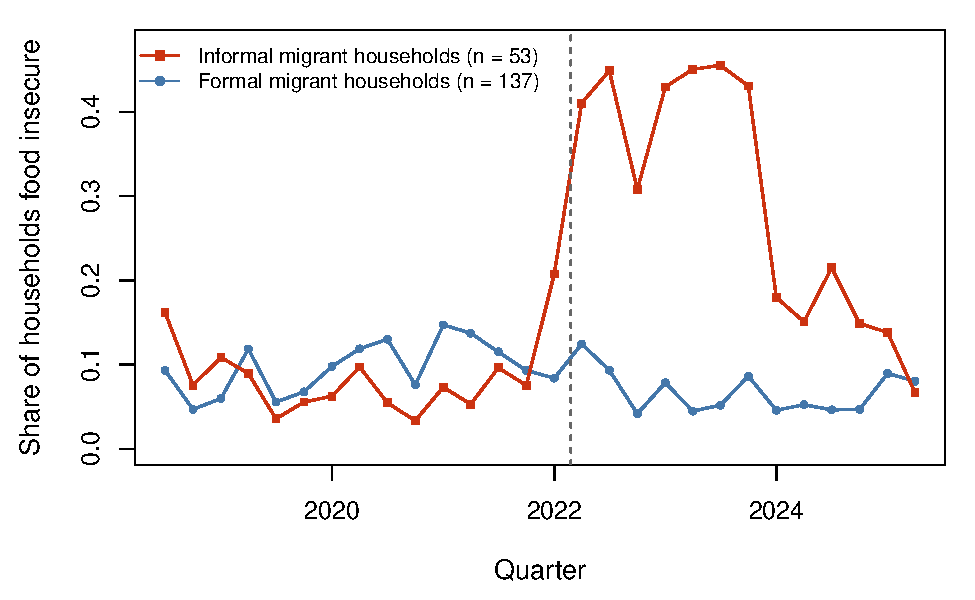
\includegraphics[width=0.85\textwidth]{figures/fig1_levels.pdf}
\caption{Food insecurity in levels, informal and formal migrant households}
\label{fig:1}
\begin{figurenotes}
The figure shows, by calendar quarter, the raw share of households that reported not being able to buy enough food in the last 30 days, separately for the informal (n = 53) and formal (n = 137) Russia migrant households classified in the baseline window (rounds 39 to 42). No control variables, weights or seasonal adjustments are applied. The dashed vertical line marks the February 2022 invasion. The series covers 82 survey rounds, September 2018 to June 2025. Source. The author's calculations from L2CU.
\end{figurenotes}
\end{figure}

Table~\ref{tab:2} reports the estimates of specification~\eqref{eq:did}. The baseline coefficient on Informal $\times$ Post is +0.279 with a clustered standard error of 0.042. Given a pre-war food insecurity level of about 9 percent across the two groups together in this sample, the estimate means that the share of informal households that could not buy enough food rose by about 28 percentage points more than in formal households. This is a very large effect. In the informal group taken on its own the raw rate rose from 7.6 to 30.8 percent, a fourfold increase, and the unadjusted difference-in-differences visible in those raw means, +0.260, is close to the regression estimate reported here (Table~\ref{tab:B10}).

\begin{table}[!ht]
\caption{The main result, food insecurity, informal and formal migrant households}
\label{tab:2}
\small
\begin{tblr}[booktabs]{width=\textwidth, rowsep=1.2pt, colspec={X[2.4,l]X[1,r]X[1,r]X[1,r]X[1,r]}}
 & (1) Baseline & (2) Weighted & (3) By phase & (4) Controls \\
\midrule
Informal $\times$ Post & +0.279*** & +0.304*** &  & +0.283*** \\
 & (0.042) & (0.046) &  & (0.041) \\
Informal $\times$ Invasion (Mar--Sep 2022) &  &  & +0.345*** &  \\
 &  &  & (0.053) &  \\
Informal $\times$ Mobilization (Oct 2022--Mar 2023) &  &  & +0.322*** &  \\
 &  &  & (0.054) &  \\
Informal $\times$ Apr--Sep 2023 &  &  & +0.451*** &  \\
 &  &  & (0.065) &  \\
Informal $\times$ Oct 2023 onwards &  &  & +0.176*** &  \\
 &  &  & (0.030) &  \\
Household fixed effects & Yes & Yes & Yes & Yes \\
Survey-round fixed effects & Yes & Yes & Yes & Yes \\
Observations & 14,128 & 14,128 & 14,128 & 14,128 \\
Households & 190 & 190 & 190 & 190 \\
\end{tblr}
\begin{tablenotes}
The dependent variable is de-seasonalized food insecurity, an indicator of not being able to buy enough food in the last 30 days. The sample covers the Russia migrant households with a baseline formality status over 82 survey rounds, September 2018 to June 2025. All specifications include household and survey round fixed effects, whose coefficients are not reported. The standard errors in parentheses are clustered at the household level. Column (2) uses the survey population weights. Column (3) replaces the single post interaction with interactions of the treatment indicator with four post-invasion phase indicators, covering survey rounds 43 to 49 (March to September 2022), 50 to 55 (October 2022 to March 2023), 56 to 61 (April to September 2023) and 62 onwards (October 2023 to June 2025), which follow the sequence described in Section~\ref{sec:3-3}, which is why the Informal $\times$ Post row is empty in that column. Round 49, September 2022, is assigned to the invasion phase, because it was in the field from 3 to 26 September and most of its interviews were completed before the mobilization was announced on 21 September. Column (4) adds interactions of the post indicator with the baseline migration channel and household education. (*** significant at the 1 percent level, ** at 5 percent, * at 10 percent.) Source. The author's calculations from L2CU.
\end{tablenotes}
\end{table}

The estimate is stable across specifications. Applying the population weights raises it to +0.304, so when households are weighted to the national population the effect is even stronger, and adding controls for the migration channel and education leaves it at +0.283. The phase decomposition in column (3) shows that the difference is present in every post-invasion period, +0.345 in the invasion phase, +0.322 in the mobilization period, a peak of +0.451 in April to September 2023, and +0.176 from October 2023 onwards, which is still large a year and a half after the shock and remains so to the end of the panel in June 2025.

A permutation test that randomly reassigns the informality label across households 2,000 times and reestimates the specification never produces an effect of this size (p < 0.001). This removes the concern that, with 53 households in the treatment group, the usual standard errors might over-reject, the result does not depend on the asymptotic approximation.

Figure~\ref{fig:2} shows the annual event study that supports identification, and Appendix Table~\ref{tab:B2} reports the same coefficients with their standard errors. The interaction coefficients are close to zero over the pre-war years, +0.067 in 2018, +0.028 in 2019 and effectively zero in 2020 ($-$0.002). The difference opens sharply at the invasion, reaching +0.301 in 2022, peaking at +0.426 in 2023, and then falling to +0.190 in 2024 and +0.083 in 2025, so it remains positive more than three years after the shock. The monthly pre-shock trend test cannot reject the parallel paths assumption ($p = 0.55$). A pooled calendar-month adjustment, which does not use the treatment label, gives a more conservative test ($p = 0.024$). The annual coefficients are flat in the years immediately before the shock, and for the reasons set out in Section~\ref{sec:6-6} the identification case rests on them rather than on the monthly test.

\begin{figure}[!ht]
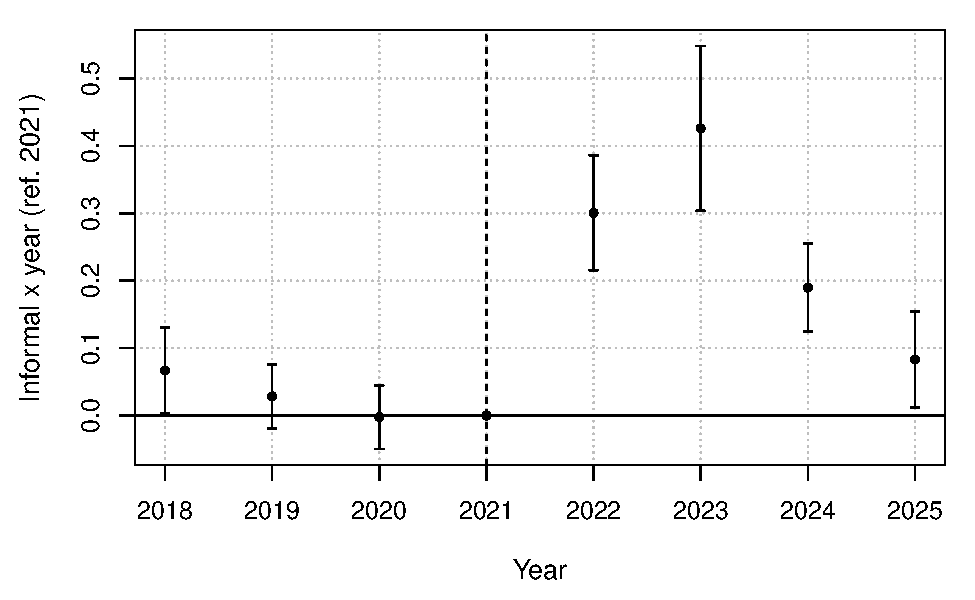
\includegraphics[width=0.85\textwidth]{figures/fig2_eventstudy.pdf}
\caption{Food insecurity, informal and formal migrant households, annual event study}
\label{fig:2}
\begin{figurenotes}
The figure shows the coefficients of the interaction of the baseline informality indicator with each calendar year, relative to 2021, from a regression of food insecurity on household and year fixed effects. The sample covers 190 Russia migrant households and 14,128 household round observations over 82 survey rounds, September 2018 to June 2025. The vertical lines show the 95 percent confidence intervals, and the standard errors are clustered at the household level. The dashed vertical line marks the February 2022 invasion. Source. The author's calculations from L2CU.
\end{figurenotes}
\end{figure}

Two features of the figure deserve emphasis. The first is the 2020 coefficient, which serves as a placebo in time. COVID-19 was a large shock for Central Asian labor migration, borders were closed, movement was restricted and activity in the service sectors that employ many migrants contracted sharply in the spring of 2020. Even so, informal and formal households did not separate in that period. The factor that made informal households vulnerable in 2022 did not make them vulnerable in 2020, which separates the finding from a general fragility that would appear in any downturn. The conceptual framework in Section~\ref{sec:4} explains this as follows. COVID reduced migrant employment in both groups by roughly the same amount, because border closures and falling demand do not sort by document, while the 2022 shock combined the labor market contraction with the mass departure caused by mobilization and with legal enforcement pressure that fell mainly on undocumented workers.

The second is the 2018 coefficient of +0.067, which stands apart because it is small but still significantly different from zero. It falls more than three years before the shock, in the sparsest early rounds of the panel, when both coverage and the relevance of a status measured at the end of 2021 were lowest. The neighboring pre-war years are clean and the formal pre-shock trend test does not reject the assumption. Section~\ref{sec:8-5} reports the check that drops these rounds.

\subsection{The damage is specific to food}\label{sec:7-3}

Table~\ref{tab:B9} extends the comparison across the welfare outcomes and applies the Romano and Wolf correction. The pattern is informative not only through what is significant but also through what is not.

Two outcomes pass both checks cleanly and a third passes with a qualification. Food insecurity passes the correction with p < 0.001. Forgone medical care passes with a corrected p of 0.017, but with a negative sign, $-$0.052, informal households gave up medical care less than formal households after the shock. Reduced food consumption passes the correction (+0.085, p = 0.024), but it should not be read as a second margin of adjustment. The raw rates fall in both groups after the shock, and the pooled estimate is driven by pre-shock differences rather than post-shock rises (pre-trend p = 0.09). Reduced food consumption is statistically significant after the Romano-Wolf correction (+0.085, corrected p = 0.024), but its pre-shock trend is comparatively weak (p = 0.09). It is therefore not treated as independent causal evidence of a post-shock adjustment margin. The main food-insecurity result does not depend on this outcome. Appendix Figure~\ref{fig:A4} shows the annual event studies for these two secondary outcomes.

Two null results are as informative as the significant ones. The water supply disruption placebo does not pass the correction (p = 0.196), which is exactly the case the procedure exists to detect, the design is not mechanically producing significant coefficients on outcomes it should not affect. The coping indicator shows the reverse case, it passes the correction easily (p = 0.002) but clearly fails the pre-shock trend test (p = 0.010), that is the two groups were already separating on coping before the war and the post-war difference cannot be attributed to it. Its negative sign, $-$0.081, would fit prediction P3, but the failed trend test means it cannot be read as an effect of the war. Together these cases show why both checks are necessary, neither test replaces the other.

The pattern across the outcomes matches prediction P4 of Section~\ref{sec:4} closely. The shock did not cause a general collapse in the welfare of informal households. It produced an adjustment concentrated in food, the most flexible item of the household budget, while committed expenses such as utilities were maintained and health spending was in fact protected. The negative coefficient on forgone medical care seems odd at first, but under a budget constraint it is the natural counterpart of the food result, a household that absorbed the income shock by cutting food is a household that chose not to absorb it by cutting medical care. This does not contradict the main finding, it identifies which margin the adjustment fell on.

\subsection{The mechanism, the migrant income channel}\label{sec:7-4}

Why exactly were the informal households hit? Section~\ref{sec:4} sets out the chain: the migrant stays employed abroad, keeps sending money, and the household keeps eating. Table~\ref{tab:B5} tests each link.

Each link moves in the direction predicted by the conceptual framework. After the shock, the migrants of informal households are less likely to be employed abroad ($-$0.099), less likely to remain abroad at all ($-$0.077), less likely to send money ($-$0.060), and send less when they do ($-$0.390 in the inverse hyperbolic sine form, although this link is the weakest of the four). The pre-shock trend tests for these variables are weak throughout. Only the presence of the migrant abroad clears the ten percent level comfortably (p = 0.23); the other four sit at or just below it, between 0.08 and 0.10. The chain is therefore identified less firmly than the food outcome, whose pre-shock trend test returns 0.55, and this is a further reason to read the mechanism as suggestive rather than established. Appendix Figure~\ref{fig:A5} plots the remittance value link month by month. Its coefficients are measured against the single round before the invasion, while the pooled estimate in Table~\ref{tab:B5} differences the whole pre-shock period against the whole post-shock period, so the two are not directly comparable in level and only the pooled estimate should be read as the effect. No link is significant on its own at usual levels, which reflects the power ceiling set by 53 households in the treatment group rather than an absence of effect. The composite indicator that combines employment abroad and sending money is significant at the 10 percent level two-sided and at 5 percent one-sided.

The intensive margin is the weakest link and deserves separate comment. Figure~\ref{fig:A5} plots it month by month over the year and a half around the invasion, and all but one coefficient in that window is positive relative to the month before the shock. The pooled estimate is negative because the pre-shock differential falls steeply through that window, from about +2.2 five months before the invasion to +0.3 immediately before it, while the post-shock differential is flat at around +0.8. The negative sign therefore reflects a decline that was already under way rather than a break at the invasion, which is what the pre-shock trend test registers at p = 0.10. The mechanism argument rests on the extensive margin and on the composite, not on the amount sent. Reestimating the composite over the progressively wider baseline windows of Section~\ref{sec:8-4} leaves the point estimate almost unchanged while the significance improves as the treatment group grows: $-$0.073 with 53 treated households, $-$0.064 with 65, $-$0.071 with 72 and 79, $-$0.061 with 85, and $-$0.066 with 89, moving from 10 percent significance in the narrowest window to 5 percent in the wider ones. The coefficient remains similar in magnitude as the treatment group expands, while the standard error falls with the larger sample. This pattern is consistent with an effect that is estimated imprecisely in the narrower samples, but it does not by itself establish the mechanism causally. What can be said with confidence is that the income channel is the only candidate mechanism that is consistent in direction across all its links and whose pre-shock trends, while weak, are not rejected as clearly as those of the alternatives.

Table~\ref{tab:B8} decomposes the composite by phase, and the timing is informative. The measurable loss of the income channel is concentrated in 2023. It is small and insignificant in the invasion phase ($-$0.032) and the mobilization phase ($-$0.059), becomes significant in April to September 2023 ($-$0.125), and then partly fades ($-$0.078). This matches the macroeconomic sequence: 2022 was a year in which remittances were strong in aggregate because of the recovering ruble, while 2023 was the period when the ruble moved to a steady decline and aggregate transfers to Uzbekistan contracted.

One further split points in the same direction. Appendix Table~\ref{tab:B4} divides the estimation sample at the median share of baseline months in which the household received a transfer. In the households above the median, the estimate is +0.467; in the households at or below it, +0.205. The households that relied on remittances most often are the ones in which the informal and formal difference is largest, which is what the income channel predicts. The subsamples are small: only 15 informal households fall in the upper group. The split is not an identified heterogeneity test, so it is reported as descriptive support rather than as evidence on its own.

Two alternative channels can be considered and set aside. Coping, that is borrowing, drawing on savings, or selling assets, fails the pre-shock trend test and is not identified as a channel. Return migration is the same. Appendix Figure~\ref{fig:A3} shows the raw series for Russia-exposed against other-destination households rather than the informal and formal split used in the test, which makes the channel impossible to identify here. Their failure means the data do not support the intuitive stories that informal households managed the shock by using up savings and assets or by bringing the migrant home. Neither channel is identified here, so prediction P3 of Section~\ref{sec:4}, that these households are buffer-constrained, is left untested rather than confirmed. The September 2022 mobilization, which sharply reduced the aggregate number of migrants, also does not explain the differential, as the split reported in Section~\ref{sec:8-5} shows.

One puzzle remains, and it is better to state it openly than to hide it. The food gap opens immediately in 2022, while the income loss is statistically visible only in 2023. Part of the explanation is statistical power: the income channel coefficients grow through 2023 and are too imprecise to detect in the early phase. But the pattern is also consistent with anticipation. In the spring of 2022, amid sanctions, currency turmoil, and an uncertain labor market outlook, households may have cut consumption not in response to a realized loss but in expectation of a worsening income flow. Under this reading, the mechanism evolved: a phase of uncertainty in 2022, followed by a realized income loss in 2023 during the subsequent period of ruble depreciation. The data cannot cleanly separate these two readings, so the timing evidence is presented as a descriptive detail around a mechanism that remains, on the whole, suggestive.

\section{Robustness}\label{sec:8}

This section tests whether the main result depends on the choices made in constructing the sample, defining the treatment or estimating the specification. The exercises are grouped by the concern each one addresses.

\subsection{Alternative definitions of informality}\label{sec:8-1}

The majority rule used to classify households with several migrants is a judgment-based choice, and it is natural to worry that the result depends on it. It does not. Classifying a household as informal if at least one of its Russia migrants in the baseline worked informally, a broader rule that raises the treatment group to 85 households, gives +0.219. Requiring all baseline migrants to be informal, a stricter rule that lowers the treatment group to 40 households, gives +0.213. The majority rule used throughout gives +0.279 with 53 treated households. All three are significant at the 1 percent level and all three pass the pre-shock trend test. Appendix Table~\ref{tab:B3} reports the three rules side by side.

The majority rule gives the largest estimate, which is expected if it measures exposure most precisely, the broader rule mixes mostly formal households into the treatment group, and the strict rule drops partly exposed mixed households. That all three lie in the narrow range from +0.213 to +0.279 shows that the finding reflects a feature of the informal and formal boundary itself, not one way of drawing it.

\subsection{Weighting, matching and permutation-based inference}\label{sec:8-2}

The estimate is robust to how the sample is weighted and matched. Applying the survey population weights gives +0.304 with a standard error of 0.046, slightly larger than the unweighted estimate, which shows that the effect does not come from households overrepresented in the sample relative to the national population. Propensity score matching gives +0.267 with a standard error of 0.046. The propensity score is estimated by logit on five baseline characteristics, the mean age of members, the highest education in the household, the share of women, household size and the baseline food insecurity rate, and each informal household is matched without replacement to its nearest formal neighbor, which gives 53 matched pairs.

The permutation test described in Section~\ref{sec:6-7} is the most important check given the small treatment group. A related question is how household-rounds with no migrant record in the individual file are treated. These are coded as zero, on the reading that a household with no migrant record has nobody abroad, working or sending in that month. Only 37 of the 14,128 household-rounds have no record at all, non-response does not move differentially between the two groups after the shock ($+$0.020, standard error 0.020, p = 0.32), and treating these observations as missing rather than zero leaves the mechanism estimates almost unchanged, at $-$0.100 for employment abroad and $-$0.073 for the composite. Randomly reassigning the informality label across the 190 households in the sample 2,000 times and reestimating each time gives a null distribution centered on zero, with a mean of +0.0005 and a standard deviation of 0.036. None of the 2,000 permutations produces an effect as large as the observed estimate, giving an empirical p-value below 0.001. The estimate under the label-free adjustment is +0.275, close to the +0.279 of the main specification. The observed estimate lies far outside the range that random assignment produces, which means the result does not rely on the asymptotic approximation behind cluster robust standard errors.

\subsection{Observable confounders}\label{sec:8-3}

The most serious concern about the design is that formality may stand in for something else about the migrant or the household. Five checks examine the observable candidates.

Controlling for the baseline migration channel, whether the migrant used formal services to arrange the migration, leaves the estimate at +0.291. This matters, because the migration channel is conceptually different from employment formality, a migrant can arrive through a formal recruitment channel and then work informally, or arrange the trip independently and obtain a patent after arrival. In the data the two are only weakly correlated (r = 0.23), which indicates that they are separate margins.

Adding household education to the same specification also leaves the estimate at +0.283 with a standard error of 0.041. Education is the second largest imbalance in Table~\ref{tab:1} and the most intuitive confounder, because households with lower education may both be more likely to have an informal migrant and less able to absorb an income shock for reasons unrelated to the migrant's legal status. The estimate changes slightly upward in the same direction as Oster result.

A stricter version of the same test restricts the comparison to migrants who used the same informal migration route, so that the difference in migration channel is removed by construction and only employment formality differs. This within channel estimate, based on 44 informal and 91 formal households, is +0.225 with a standard error of 0.045. The effect is a little smaller, which is expected from a more homogeneous comparison, but it is still large and significant.

Finally, controlling for the interaction of the baseline share of women with the post indicator, the largest demographic imbalance in Table~\ref{tab:1}, leaves the estimate at +0.285 with a standard error of 0.042, and the gender term itself is insignificant (p = 0.34). The imbalance is real, but it does not drive the result.

Domestic wage income, the remaining imbalance in Table~\ref{tab:1}, is treated the same way. Controlling for the interaction of baseline wage income with the post indicator leaves the estimate at +0.274 with a standard error of 0.041, and the wage term itself is insignificant (p = 0.16).

The observable controls can also be used to say something about the unobservable ones. Following \cite{oster2019}, the movement of the coefficient when controls are added, together with the change in the explained variation, indicates how strong selection on unobservables would have to be, relative to selection on observables, for the true effect to be zero. Adding all six baseline controls jointly, each interacted with the post indicator, moves the estimate from +0.279 to +0.286 and raises the explained variation only slightly, from 0.234 to 0.239. The estimate therefore moves away from zero, not towards it, when the observable differences between the two groups are taken into account. The implied ratio is negative, about $-$2.3 when the maximum explained variation is set at 1.3 times the controlled value, which is the convention in that literature. The reading is that the pattern of selection on unobservables required to eliminate the estimated effect would have to differ substantially from the selection pattern implied by the observed characteristics. This is supportive evidence against a simple observable-selection explanation.

The confounder that cannot be tested directly is the migrant's sector of work, which the survey does not record. Informal migrant employment is known to concentrate in construction and lower end services, so if those sectors shrank more than others, the estimated difference would reflect sectoral exposure rather than legal vulnerability. Aggregate evidence makes this interpretation less likely, and it does so in the relevant direction. Construction, where informal Central Asian migrants are most represented, did not contract after the invasion but expanded. According to Rosstat, the volume of construction work rose by about 5 percent in 2022 and by a further 8 percent in 2023, helped by state subsidised mortgage programs and by domestic capital seeking shelter from the sanctions \parencite{rosstat}. If informal migrants were mostly employed in construction, sectoral exposure would predict that their households did better, not worse, so the sectoral composition is more likely a reason the estimate is pulled toward zero than the source of the result. This argument is suggestive rather than decisive, because each migrant's sector is not observed and informal workers are also present in retail and hospitality, where the exit of Western companies reduced activity. Even so, it shifts the burden of proof, a sectoral explanation would have to rest on the sharp contraction of the smaller sectors where migrants are concentrated at a time when the largest such sector was growing.

\subsection{The baseline assignment window}\label{sec:8-4}

The treatment group of 53 households is small, and the reason is the four round baseline window: a longer window classifies more households but measures status further from the shock. Appendix Table~\ref{tab:B1} reports what happens when the window is widened step by step from four to twenty-two rounds, reassigning the treatment and control groups each time. Twenty-two rounds is the practical limit, because the formality question enters the questionnaire only in round 21.

The estimate barely changes. Widening the window raises the treatment group from 53 to 89 households, that is, by two thirds, while the coefficient stays in the narrow range from +0.252 to +0.279, significant at the 1 percent level everywhere, with pre-shock trend tests that do not reject parallel trends, and the standard errors fall from 0.042 to 0.035 as the sample grows.

Two conclusions follow. First, the main result is not an artifact of the narrow baseline window or of the 53 households it selects. Second, the slight fall in the estimate observed as the window widens is itself consistent with the possibility that measuring employment status further from the shock introduces additional classification noise. The robustness exercise cannot establish that measurement error is the reason for the decline, but the stability of the estimates supports retaining the four-round window as the main specification because it provides the closest measurement of employment status to the shock.

\subsection{Time and placebo checks}\label{sec:8-5}

Three exercises complete the set of checks, each testing whether the effect sits where interpretation requires.

The COVID placebo asks whether informal households are simply worse off in any crisis. In the annual event study, the 2020 interaction is $-$0.002, informal and formal households did not separate at all during the pandemic that closed borders and sharply reduced migrant employment. This separates the finding from a general vulnerability explanation that could not be ruled out by control variables alone.

The mobilization check asks whether the effect is really tied to the September 2022 mobilization, the most visible single event of the post-shock period. Splitting the post-shock period at round 50, the first round that was entirely in the field after the announcement of 21 September 2022, gives +0.344 before it and +0.262 after. The effect neither starts nor jumps sharply at the mobilization, it is already large in the seven months before it and slightly smaller after. The factor that produced the differential was already at work before the mobilization occurred.

The early panel check examines the 2018 coefficient that stands apart in Figure~\ref{fig:2}. Dropping the 2018 rounds entirely and reestimating from 2019 leaves the estimate at +0.283 with a standard error of 0.041, effectively the same as the main specification. The 2018 coefficient may reflects a group-specific seasonal difference rather than a pre-existing separation. That year enters the annual specification with only four months, September to December, so the averaging that removes within-year seasonality in the complete years does not do so here, and the estimate barely moves when the year is dropped.

\section{Limitations}\label{sec:9}

Four limits of this analysis should be stated openly, not as afterthought caveats but as features of the data and the design. Each is a real limitation, and in each case it should be clear what it puts in doubt and what it does not.

Internal validity: the central, untestable confounder. The survey records whether the migrant works formally, but not which sector the migrant works in or which region of Uzbekistan the household is from. Informal migrant employment is known to concentrate in certain sectors, especially construction and lower end services and these sectors were not harmed equally by the 2022 shock. If informal migrants were mostly employed in the sectors that were hit hardest, the estimated difference would reflect sectoral exposure alongside legal vulnerability. The same reasoning applies to the region of origin, because regions differ in migration networks and in exposure to the corridor.

The checks in Section~\ref{sec:8-3} narrow this concern without removing it: the migration channel, education and gender composition do not explain the result, the COVID placebo argues against a general fragility reading, the sensitivity calculation implies that the selection on unobservables required to eliminate the estimated effect would have to differ substantially from the selection pattern implied by the observed characteristics, and the aggregate evidence on construction points away from a sectoral explanation rather than towards one. None of this identifies the sector or the region directly, because these variables are not in the data. The honest statement is that the estimate captures the effect of the informal work bundle, in which legal vulnerability under the patent system is the leading component but is not proven to be the only one, and that resolving this would require data linking migrants to their occupations in the destination country, which the L2CU instrument does not collect.

The mechanism is suggestive, not proven. Each link of the income chain points in the predicted direction, the composite is significant one-sided, and the phase decomposition matches the fall of the ruble, although the pre-shock trend tests for these variables are weak. But in the preferred specification the composite is only marginally significant two-sided and no single link passes the usual thresholds. With 53 households in the treatment group this is not a fault that a better specification can fix, it is a power ceiling. The defensible claim is that the income channel is consistent in direction and is the candidate mechanism that the data reject least, not that its operation is proven.

External validity: the reach of the estimate is limited. The treatment group is 53 households that experienced one shock in one country. Applying the population weights improves representativeness within Uzbekistan, but generalization to other corridors or other crises requires caution. In this respect the COVID placebo is a useful warning, it shows that not every large shock that touches migration splits households along the formality boundary. Whether the 2022 result generalizes depends on whether a future shock combines a labor market contraction with legal enforcement pressure in the same way.

The common effects are invisible by construction. The survey round fixed effects absorbs everything common to both groups. This includes any harm the war did to formal migrant households and the aggregate decline in remittances to Uzbekistan from 2023. So the estimates are differential effects, and the total welfare footprint of the shock is larger than the numbers reported here. A difference-in-differences design can identify who was hit harder, it cannot identify how much everyone was hit. Recovering the common component would require a different design, such as a shift share approach that uses cross sectional variation in exposure intensity.

\section{Conclusion}\label{sec:10}

This thesis studied how the 2022 Russian crisis affected household welfare in Uzbekistan, a country where a large part of families depends on the remittances sent by migrants working in Russia. The answer depends entirely on whether one looks at the average or at the distribution.

The average indicates resilience. Comparing households whose migrants worked in Russia with households whose migrants worked in other countries, the estimated effect on food insecurity is +0.027 with a standard error of 0.026, it does not differ from zero and the pre-shock trends do not reject parallel trends. 

The distribution shows something else. Splitting migrant households by whether the migrant held a patent, the work permit that makes employment formal and residence legal in Russia, breaks the near zero average into two very different experiences. In households whose migrant worked informally, food insecurity rose after the invasion from about 8 percent before the war to a peak above 40 percent. Relative to formal migrant households the estimated increase is about 28 percentage points, and the difference was still visible more than three years after the shock. Among households whose migrant worked formally there is no statistically detectable differential deterioration relative to their pre-war path, over and above the changes common to both groups. The line that split the households was not migration itself, but the formality of employment.

The finding rests on a design with a single common treatment date, a predetermined treatment assignment, and a pre-shock period of three and a half years over which the two groups tracked each other closely. The informal and formal difference is effectively zero in the COVID year, which separates it from a general tendency of informal households to be worse off in any crisis.

The damage is not general but specific. It is concentrated in food, the most flexible item of the household budget, while households did not become more likely to report forgone medical care; if anything, the probability of forgone care declined relative to the formal group. This is consistent with households protecting medical care relative to food, although the result should not be interpreted as a direct measure of health expenditure.

The evidence on the mechanism points to the migrant's income channel. Informal migrants were more likely to lose their work abroad and, with it, their remittances. The intuitive alternatives are not confirmed: coping and return migration fail the pre-shock trend test, and the September 2022 mobilization does not explain the informal and formal difference. The composite estimate is only marginally significant, so it is presented as suggestive rather than proven. The main limitation is not whether the difference is caused by something but what the treatment label stands for: the survey does not record the migrant's sector of work or region of origin, so the estimate identifies the effect of the informal work bundle, of which legal vulnerability under the patent system is the leading component but not demonstrably the only one.

These results answer the literature reviewed in Section~\ref{sec:2} directly. \cite{yang2007} established that remittances insure origin households against shocks at home, offsetting about 60 percent of lost domestic income and leaving consumption in migrant households largely unchanged. The findings here identify the condition under which that insurance fails. It holds when the shock reaches the household and the migrant absorbs it, and it breaks when the shock reaches the migrant himself, and the extent of the break depends on the migrant's position in the destination labor market. \cite{shimizutani2021} studied the same region during the COVID-19 pandemic with a comparable monthly panel and found that households with a migrant were more resilient than those without. Applying the same comparison to the 2022 shock gives no result, and the COVID placebo in Section~\ref{sec:7-2} shows why these two results are not in conflict, the pandemic did not split migrant households along the formality boundary, while the war did. Both their resilience result and the null result reported here are averages over an internally heterogeneous category.

Two conclusions follow.

From a policy point of view, formalizing labor migration is not only a legal or an administrative matter. In this episode formal employment abroad, resting on Russia's patent system, may have functioned as insurance for the household at home. Bilateral labor agreements, organized recruitment schemes and measures that reduce the cost of obtaining and keeping a work permit are usually justified in terms of migrants' rights or of tax compliance in the destination country, and the evidence here shows that they are at the same time instruments of social protection for the families the migrants left behind, working at a distance and before the shock. It also gives social protection systems in the origin country a clear target, because the households of informal migrants can be identified even before a shock in the destination country occurs.

From a research point of view, the practical lesson is that aggregate null results in this literature should be checked for composition before they are declared as evidence of resilience. A null result can reflect genuine protection or offsetting heterogeneity, and the margin that mattered here was not whether the household has a migrant, but what status that migrant held.

Three directions for future research follow directly from the limitations. With data that record the migrant's sector and region of origin, the remaining confounder concern could be tested rather than argued. A larger sample of informal migrant households would give the power to establish the income channel mechanism that this data can only suggest. The aggregate side of the episode, the general decline in remittances from 2023 that the differential design absorbs by construction, could be studied with methods built for common shocks, such as shift share designs that use variation in the intensity of corridor exposure. The 2022 crisis will not be the last shock to travel along the migration corridor, and understanding whom it harms, and why, makes it possible to anticipate the next one.